%Thanks to Prof. Bazioch for the use of his template
%TeXMaker on a PC or Linux and TeXShop on a mac are good editors for
%creating LaTeX documents
%A good place to get started with LaTeX is
%http://ctan.mirrors.hoobly.com/info/Math_into_LaTeX-4/Short_Course.pdf
\documentclass[12pt]{article}
\usepackage{amsmath,amssymb,amsthm}
\usepackage{graphicx}

\usepackage{enumerate,multicol,verbatim}
\usepackage{fullpage}

\setlength{\parindent}{0in}
\setlength{\parskip}{3mm}
\newcommand{\nline}{\rule{\linewidth}{0.5pt}}

\theoremstyle{plain}
\newtheorem{theorem}{Theorem}
\newtheorem{lemma}[theorem]{Lemma}
\newtheorem{proposition}[theorem]{Proposition}
\newtheorem{corollary}[theorem]{Corollary}

\theoremstyle{definition}
\newtheorem{definition}[theorem]{Definition}
\newtheorem{notation}[theorem]{Notation}
\newtheorem{remark}[theorem]{Remark}
\newtheorem{note}[theorem]{Note}
\newtheorem{nn}[theorem]{}



% document title YOU DO NOT NEED TO CHANGE THIS
\makeatletter
\renewcommand{\maketitle}{
\begin{center}
\nline\\
\vspace{2ex}
{\huge \textsc{\@title}}
\nline\\
{\large\textsc{\@author \hfill \@date}}
\vspace{4ex}
\end{center}
}
\makeatother
%%%

%%%%%%%%%%%%%%%%%%%%%%%%%%%%%%%
%%%%%%%%%%%%%%%%%%%%%%%%%%%%%%%

%%%%%%% THIS SHOULD BE CHANGED FOR EACH NEW ASSIGNMENT

\title{HPC I Homework 1}

%%%%%%% BE SURE TO PUT IN YOUR OWN NAME

\author{Morse, Michael}

%%%%%%% BE SURE TO PUT IN THE DUE DATE

\date{October 5, 2017}

%%%%%%%%%%%%%%%%%%%%%%%%%%%%%%%
%%%%%%%%%%%%%%%%%%%%%%%%%%%%%%%


\begin{document}

\maketitle

%%%%%%%%%%%%%%%%%%%%%%%%%%%%%%%
%Problem 1
%%%%%%%%%%%%%%%%%%%%%%%%%%%%%%%

\section*{Problem 1}
For this problem, run squeue $>$ queue.txt and query this text file (using cat) to answer
the following questions. Submit queue.txt with your answers. Construct one-liners to
answer the following questions. Submit both the command you used and the answer.

As discussed in lecture there is a bash script that writes this information. I have copied the output of the bash script here\\
What user has the most pending jobs and how many are there? \\
665 yudhajit\\
How many total nodes is this user using?\\
665\\
Which user, that has a running job, has the longest username?\\
8 zhixuanc\\
What is the largest number of nodes being utitlized and by what user?\\
mohsenda 40\\
How many unique users have pending jobs because of priority?\\
7

\section*{Problem 2}

\begin{figure}
\label{fig:problem2}
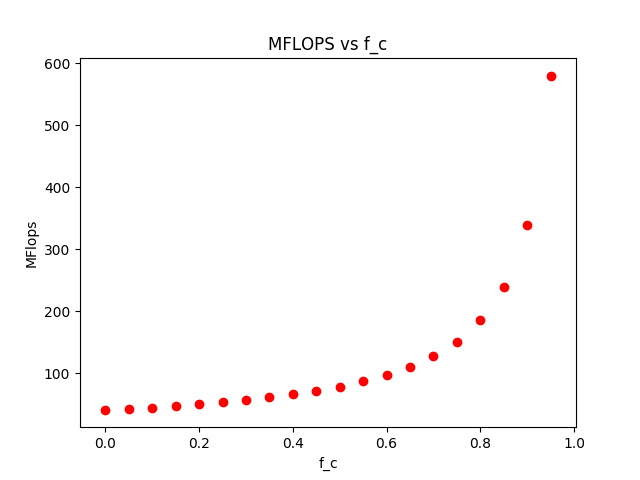
\includegraphics[scale=0.7]{problem2.png}
\caption{Problem 2}
\end{figure}
I have included a plot of performance as a function of $f_c$ for the requested values we have
\subsection{$f_c = 0.01$}
predicted performance is 40.40 MFLOPS
\subsection{$f_c = 0.99$}
predicted performance is 1342.28 MFLOPS

\section*{Problem 3}
Write a program to perform matrix addition C = A +B for $n \times n$ matrices for various $n$,
up to $n = 10000$ or $n = 20000$ depending on how much memory the machine has. Time
the addition procedure first looping over rows, then columns and vice-versa. Experiment
with different optimization options. Try both Intel compilers and GCC compilers (use
newer GCC’s, available as modules on CCR). Report your results. Do you see a difference
in time between the loop orders? Explain.

\begin{figure}
\label{fig:problem3}
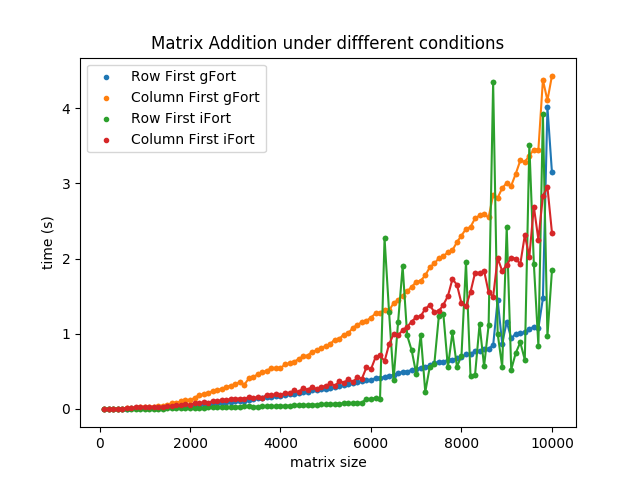
\includegraphics[scale=0.7]{problem3.png}
\caption{Matrix addition with different compilers and ordering}
\end{figure}

As can be seen from figure \ref{fig:problem3} for both iFort and gfortran  column fist matrix addition is significantly less efficient than the row first ordering. This is likely because Fortran stores two dimensional arrays down columns. So if we sum over rows first the compiler is able to optimize on this by grabbing an entire column at a time. For a single instruction of $C(i,j) = A(i,j) + B(i,j)$ the compiler can grab say $j,j+1,j+2,j+3$ filling up the cache on a for a single memory access as they are in the same column and stored next to each other. When sum over columns first the next element to be added is not stored next to the previous so the compiler can not grab multiple pieces of data at the same time to preform the operation on. We also notice the vectorization makes the process much much faster for the row first ordering. With the Intel compiler under -O3 optimization the size $10^4$ matrices are added in times comparable to  size $10^3$ matrices row first process under gfortran.

 
\section*{Problem 4}
Write a program that implements a vector dot product (L1 BLAS function). Reproduce
the performance plot from the architecture lecture. Look in the /proc/cpuinfo file in
order to be able to compute theoretical peak performance. Experiment with optimizations.
What percentage of peak performance do you achieve? Can you explain the results
you see on the performance plot?
Now compare with the standard Netlib BLAS function ddot by writing a program that
calls this function and links against the blas library (either CCR’s native blas library in
/lib64 or you can download from netlib and build yourself).
Finally, compare against the optimized version of ddot in the MKL library (use the
environment modules to load MKL and for instructions on linking).

\begin{figure}  
\label{fig:problem4}
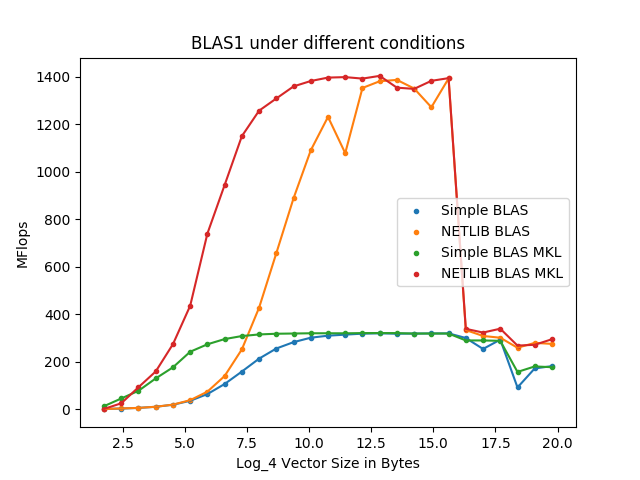
\includegraphics[scale=0.7]{problem4.png}
\caption{BLAS1 with different conditions}
\end{figure}

For the ccr rush machine the theoretical peak performance is 68,000 MFlops. For a simple BLAS1 scalar product function we achieve a max performance of around 300MFlops or 0.4\% of peak. MKL library did not improve this. For the NETLIB Blas we achieved a max performance of 1400 MFLOPS or 2 \% of peak. We notice that while MKL did not improve the peak performance MKL did achieve peak faster and preformed better for all sizes where $n < 4 *10^6$. We also see a nice drop-off around a size of about $4^{12}$ Bytes of array sizes of 16MB corresponding to the point where the on cache is filled and we start having to pull from off chip cache. The cache on rush is 24MB so at this point we can no longer load both arrays to cache on chip. We also see a massive drop at $4^{15}$ or about 1GB where now the main memory is being used and the process slows way down.

\section*{Problem 5}
Write a program that implements a vector dot product (L1 BLAS function). Reproduce
the performance plot from the architecture lecture. Look in the /proc/cpuinfo file in
order to be able to compute theoretical peak performance. Experiment with optimizations.
What percentage of peak performance do you achieve? Can you explain the results
you see on the performance plot?
Now compare with the standard Netlib BLAS function ddot by writing a program that
calls this function and links against the blas library (either CCR’s native blas library in
/lib64 or you can download from netlib and build yourself).
Finally, compare against the optimized version of ddot in the MKL library (use the
environment modules to load MKL and for instructions on linking).

\begin{figure}  
\label{fig:problem5}
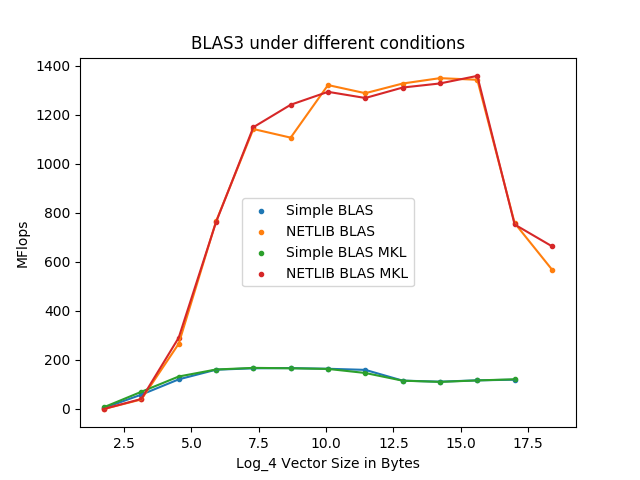
\includegraphics[scale=0.7]{problem5.png}
\caption{BLAS3 with different conditions}
\end{figure}

For the ccr rush machine the theoretical peak performance is 68,000 MFlops. For a simple BLAS3 matrix matrix multiplication function we achieve a max performance of around 200MFlops or 0.3\% of peak. MKL library did not improve this. For the NETLIB BlAS we achieved a max performance of 1400 MFLOPS or 2 \% of peak. Here we remark that while this process seems like it should take much longer than the problem 4 scalar product as the number of operations go like $\mathcal{O}(n^3)$ instead of $\mathcal{O}(n)$. However we notice this does not happen. For matrices and vectors of comparable size in Bytes the speed of these two processes are comparable. We notice that while MKL echoed the results of the non MKL routines. For the BLAS3 I also ran MKL with ifort to compare intels libraries compiled under ifort and gfortan. We notice in figure \ref{fig:problem5} that the simple BLAS 3 routine compiled with Intel's Fortran compiler peaks at around 1500 MFLOPS or 2.2\% of peak before falling off faster than the NETLIB BLAS routines under either compiler.  

\end{document}
